\documentclass{sigchi}

% Use this section to set the ACM copyright statement (e.g. for
% preprints).  Consult the conference website for the camera-ready
% copyright statement.

% Copyright
\CopyrightYear{2020}
%\setcopyright{acmcopyright}
\setcopyright{acmlicensed}
%\setcopyright{rightsretained}
%\setcopyright{usgov}
%\setcopyright{usgovmixed}
%\setcopyright{cagov}
%\setcopyright{cagovmixed}
% DOI
\doi{https://doi.org/10.1145/3313831.XXXXXXX}
% ISBN
\isbn{978-1-4503-6708-0/20/04}
%Conference
\conferenceinfo{CHI'20,}{April  25--30, 2020, Honolulu, HI, USA}
%Price
\acmPrice{\$15.00}

% Use this command to override the default ACM copyright statement
% (e.g. for preprints).  Consult the conference website for the
% camera-ready copyright statement.

%% HOW TO OVERRIDE THE DEFAULT COPYRIGHT STRIP --
%% Please note you need to make sure the copy for your specific
%% license is used here!
% \toappear{
% Permission to make digital or hard copies of all or part of this work
% for personal or classroom use is granted without fee provided that
% copies are not made or distributed for profit or commercial advantage
% and that copies bear this notice and the full citation on the first
% page. Copyrights for components of this work owned by others than ACM
% must be honored. Abstracting with credit is permitted. To copy
% otherwise, or republish, to post on servers or to redistribute to
% lists, requires prior specific permission and/or a fee. Request
% permissions from \href{mailto:Permissions@acm.org}{Permissions@acm.org}. \\
% \emph{CHI '16},  May 07--12, 2016, San Jose, CA, USA \\
% ACM xxx-x-xxxx-xxxx-x/xx/xx\ldots \$15.00 \\
% DOI: \url{http://dx.doi.org/xx.xxxx/xxxxxxx.xxxxxxx}
% }

% Arabic page numbers for submission.  Remove this line to eliminate
% page numbers for the camera ready copy
% \pagenumbering{arabic}

% Load basic packages
\usepackage{balance}       % to better equalize the last page
\usepackage{graphics}      % for EPS, load graphicx instead 
\usepackage[T1]{fontenc}   % for umlauts and other diaeresis
\usepackage{txfonts}
\usepackage{mathptmx}
\usepackage[pdflang={en-US},pdftex]{hyperref}
\usepackage{color}
\usepackage{booktabs}
\usepackage{textcomp}
\usepackage{pdflscape}
\usepackage{afterpage}
\usepackage{capt-of}

\usepackage{pgfgantt}
\usepackage{pdflscape}

\definecolor{barblue}{RGB}{153,204,254}


% Some optional stuff you might like/need.
\usepackage{microtype}        % Improved Tracking and Kerning
% \usepackage[all]{hypcap}    % Fixes bug in hyperref caption linking
\usepackage{ccicons}          % Cite your images correctly!
% \usepackage[utf8]{inputenc} % for a UTF8 editor only

% If you want to use todo notes, marginpars etc. during creation of
% your draft document, you have to enable the "chi_draft" option for
% the document class. To do this, change the very first line to:
% "\documentclass[chi_draft]{sigchi}". You can then place todo notes
% by using the "\todo{...}"  command. Make sure to disable the draft
% option again before submitting your final document.
\usepackage{todonotes}

% Paper metadata (use plain text, for PDF inclusion and later
% re-using, if desired).  Use \emtpyauthor when submitting for review
% so you remain anonymous.
\def\plaintitle{SIGCHI Conference Proceedings Format}
\def\plainauthor{First Author, Second Author, Third Author,
  Fourth Author, Fifth Author, Sixth Author}
\def\emptyauthor{}
\def\plainkeywords{Authors' choice; of terms; separated; by
  semicolons; include commas, within terms only; this section is required.}
\def\plaingeneralterms{Documentation, Standardization}

% llt: Define a global style for URLs, rather that the default one
\makeatletter
\def\url@leostyle{%
  \@ifundefined{selectfont}{
    \def\UrlFont{\sf}
  }{
    \def\UrlFont{\small\bf\ttfamily}
  }}
\makeatother
\urlstyle{leo}

% To make various LaTeX processors do the right thing with page size.
\def\pprw{8.5in}
\def\pprh{11in}
\special{papersize=\pprw,\pprh}
\setlength{\paperwidth}{\pprw}
\setlength{\paperheight}{\pprh}
\setlength{\pdfpagewidth}{\pprw}
\setlength{\pdfpageheight}{\pprh}

% Make sure hyperref comes last of your loaded packages, to give it a
% fighting chance of not being over-written, since its job is to
% redefine many LaTeX commands.
\definecolor{linkColor}{RGB}{6,125,233}
\hypersetup{%
  pdftitle={\plaintitle},
% Use \plainauthor for final version.
%  pdfauthor={\plainauthor},
  pdfauthor={\emptyauthor},
  pdfkeywords={\plainkeywords},
  pdfdisplaydoctitle=true, % For Accessibility
  bookmarksnumbered,
  pdfstartview={FitH},
  colorlinks,
  citecolor=black,
  filecolor=black,
  linkcolor=black,
  urlcolor=linkColor,
  breaklinks=true,
  hypertexnames=false
}


\definecolor{barblue}{RGB}{153,204,254}
\definecolor{groupblue}{RGB}{51,102,254}
\definecolor{linkred}{RGB}{165,0,33}
\renewcommand\sfdefault{phv}
\renewcommand\mddefault{mc}
\renewcommand\bfdefault{bc}
\setganttlinklabel{s-s}{START-TO-START}
\setganttlinklabel{f-s}{FINISH-TO-START}
\setganttlinklabel{f-f}{FINISH-TO-FINISH}
\sffamily


% create a shortcut to typeset table headings
% \newcommand\tabhead[1]{\small\textbf{#1}}

% End of preamble. Here it comes the document.
\begin{document}

\title{Developing an affect enhanced "Turrellian" RGB LED lamp designed to improve mood: towards multimodal affect-sensitive computing and devices.}

\numberofauthors{2}
\author{
\alignauthor{Humphrey Curtis\\
\email{dr19500@bristol.ac.uk}}\\
\affaddr{Supervised by Dr Paul O'Dowd}\\
\affaddr{University of Bristol, United Kingdom}\\
}


\maketitle

\section{Executive Summary}
This proposal presents potential insights from building and user experience (UX) testing an affect-enhanced RGB LED lamp, which utilises tightly synchronised body sensors and a self-journaling application to gauge users’ affective signals. The RGB LED lamp fundamentally differs from other smart-lighting internet of things (IoT) devices because it is the first device to be tethered to users’ affective state and be designed to offer mood enhancement utilising research from colour psychologists Valdez et al.~\cite{valdez1994effects}. Inspired by the work of lightscape artist James Turrell, the LED lamp is designed to bridge the gap between mindful applications and smart lighting systems – improving users’ day-to-day quality of life. Additionally, this device will contribute to academic research within multimodal affect-sensitive computing. Emotional intelligence is a facet of human intelligence that has been argued to be indispensable and perhaps most important for successful interpersonal social interaction. A wide variety of cues have been used by multimodal human computer interaction (MHCI) researchers to determine user’s emotion such as facial expression, body movements, vocal expressions and physiological reactions. However, this proposal offers strong support and insights for embodied and physiological (tacticle) approaches towards affect-sensing systems and multimodal device design.


% ACM Classfication


\begin{CCSXML}
<ccs2012>
<concept>
<concept_id>10010583.10010588.10010596</concept_id>
<concept_desc>Hardware~Sensor devices and platforms</concept_desc>
<concept_significance>300</concept_significance>
</concept>
<concept>
<concept_id>10010405.10010455.10010459</concept_id>
<concept_desc>Applied computing~Psychology</concept_desc>
<concept_significance>500</concept_significance>
</concept>
<concept>
<concept_id>10010405.10010406.10010422</concept_id>
<concept_desc>Applied computing~Event-driven architectures</concept_desc>
<concept_significance>500</concept_significance>
</concept>
<concept>
<concept_id>10010147.10010178.10010187</concept_id>
<concept_desc>Computing methodologies~Knowledge representation and reasoning</concept_desc>
<concept_significance>500</concept_significance>
</concept>
<concept>
<concept_id>10010147.10010178.10010179</concept_id>
<concept_desc>Computing methodologies~Natural language processing</concept_desc>
<concept_significance>500</concept_significance>
</concept>
<concept>
<concept_id>10003120.10003138</concept_id>
<concept_desc>Human-centered computing~Ubiquitous and mobile computing</concept_desc>
<concept_significance>500</concept_significance>
</concept>
<concept>
<concept_id>10003120.10003121.10003122</concept_id>
<concept_desc>Human-centered computing~HCI design and evaluation methods</concept_desc>
<concept_significance>500</concept_significance>
</concept>
<concept>
<concept_id>10002951.10003317.10003371.10003386</concept_id>
<concept_desc>Information systems~Multimedia and multimodal retrieval</concept_desc>
<concept_significance>500</concept_significance>
</concept>
<concept>
<concept_id>10002951.10003317.10003371.10010852</concept_id>
<concept_desc>Information systems~Environment-specific retrieval</concept_desc>
<concept_significance>500</concept_significance>
</concept>
<concept>
<concept_id>10002951.10003317.10003347.10003353</concept_id>
<concept_desc>Information systems~Sentiment analysis</concept_desc>
<concept_significance>500</concept_significance>
</concept>
</ccs2012>
\end{CCSXML}

\ccsdesc[300]{Hardware~Sensor devices and platforms}
\ccsdesc[500]{Applied computing~Psychology}
\ccsdesc[500]{Applied computing~Event-driven architectures}
\ccsdesc[500]{Computing methodologies~Knowledge representation and reasoning}
\ccsdesc[500]{Computing methodologies~Natural language processing}
\ccsdesc[500]{Human-centered computing~Ubiquitous and mobile computing}
\ccsdesc[500]{Human-centered computing~HCI design and evaluation methods}
\ccsdesc[500]{Information systems~Multimedia and multimodal retrieval}
\ccsdesc[500]{Information systems~Environment-specific retrieval}
\ccsdesc[500]{Information systems~Sentiment analysis}


\section{Introduction}

Computing technologies will increasingly embed themselves into the fabric of our everyday living spaces and project the human user into the foreground~\cite{6634207}. Therefore, computer systems and devices will become more user-centric and intelligent – seamlessly serving the needs of the user with software operating automatically in the background. Indeed, advances in computing power, wearable computer devices and interaction modalities promises a new dawn for MHCI systems and applications. Consequently, Pantic et al. encouraged the development of multimodal computing (or HCI2) – specifically computing which can understand and respond to natural and autonomic modes of human communication such as emotion automatically~\cite{pantic2008human, 6634207}.

\begin{figure*}
  \centering
  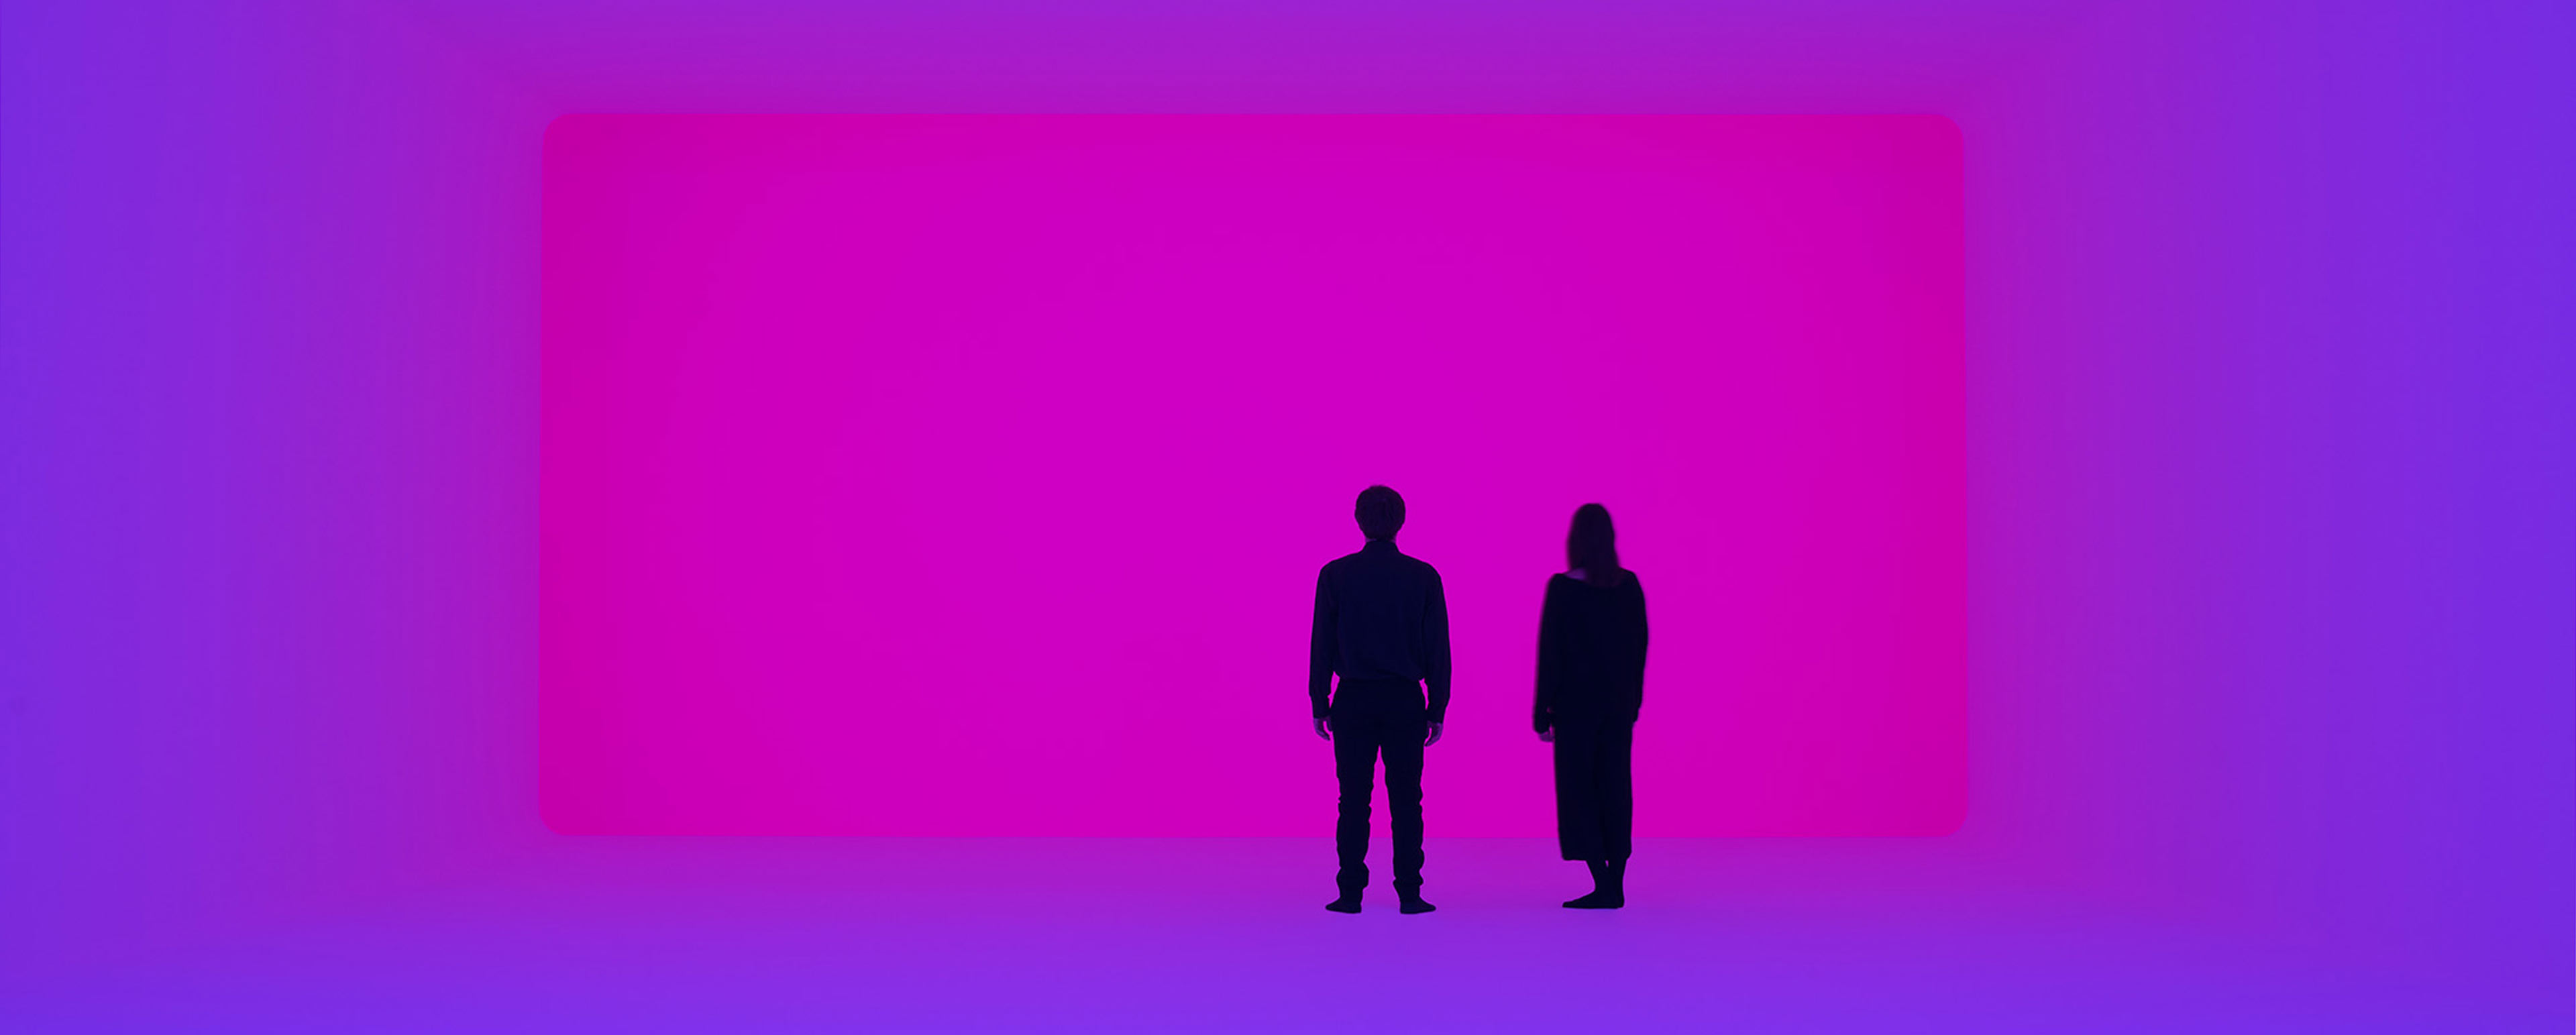
\includegraphics[width=1.75\columnwidth]{figures/turrell}
  \caption{In this immersive installation titled, "Aural" James Turrell demonstrates the immersive qualities of programmed LED lighting and the Ganzfeld effect. Exhibited at the Jewish Museum, Berlin (April 2018 - October 2019).}~\label{fig:figure1}
\end{figure*}


\begin{figure}
\centering
  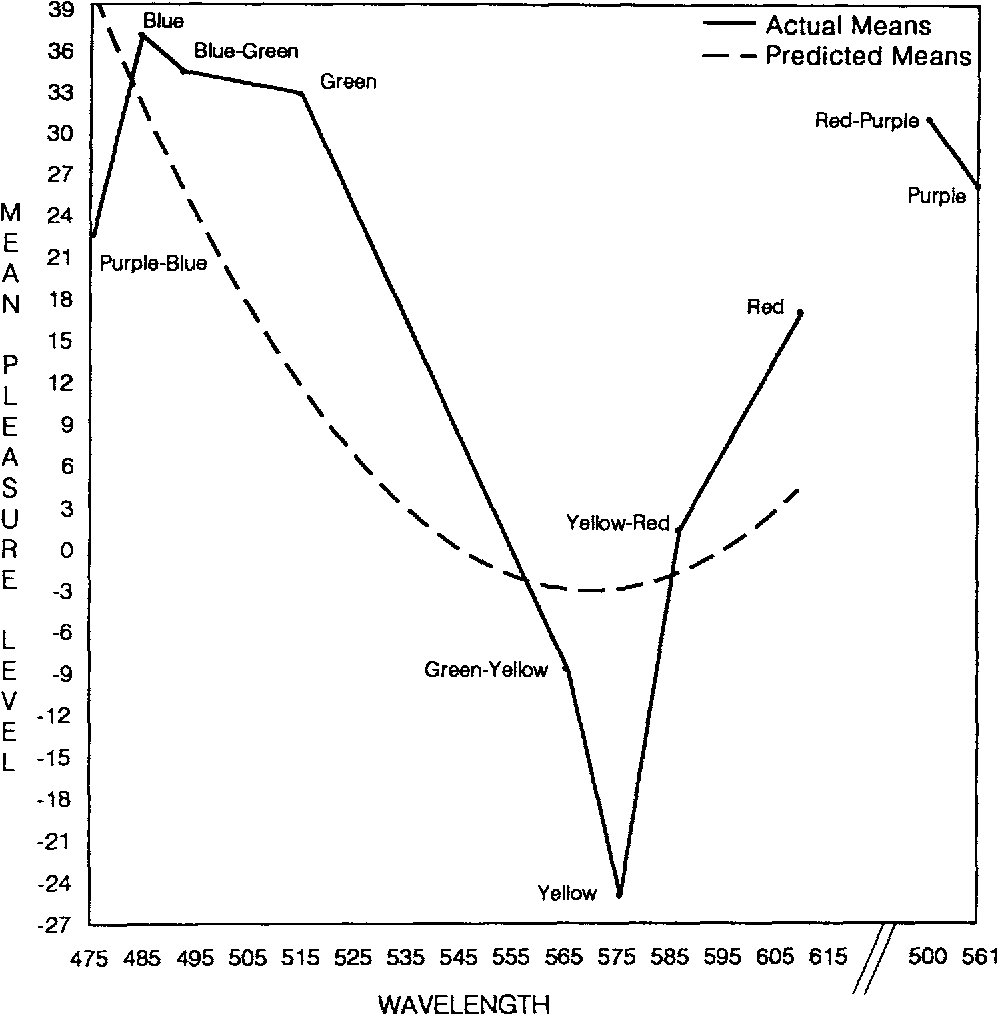
\includegraphics[width=0.9\columnwidth]{figures/Valdez}
  \caption{Some of Valdez et al.'s data demonstrating the significance of colour and wavelength on stimulating pleasure and arousal.}~\cite{valdez1994effects}~\label{fig:figure2}
\end{figure}


\subsection{Motivation}

Since Pantic et al.'s paper in 2008, affective computing has experienced much research interest – particularly developing affect-sensitive multimodal computer interfaces and operating systems~\cite{pantic2008human, 5771346}. Yet, subsequently, MHCI researcher’s emotion recognition methodologies have differed greatly (see literature review). Consequently, at present, MHCI affective-computing research has not reached consensus in multiple areas. This paper will develop a Turrellian RGB LED lamp designed to improve user’s mood in order to add to the academic debate and provide insights for future affective computing research. Therefore, this paper has two key motivations. Firstly, to design, engineer and evaluate an affect-enhanced RGB LED lamp for UX testing. Secondly, to utilise the devices’ findings to provide further research into developing successful multimodal affect-sensitive computer systems.

Computer and IoT retail markets have seen several light devices for example, the Phillips Energy Up~\cite{Phillips01}, Lumie Bodyclock~\cite{Lumie01} and Dodow~\cite{Dodow01} created to treat disorders and syndromes such as seasonal affective disorder (SAD), sleep disorders and even dementia. However, these devices are manually calibrated by their users or medical practitioners to treat a specific health problem and there is no concrete evidence of their effect on improving user’s mood. Consequently, at present there is no lighting device or computer system calibrated to improve overall mood, engender positive emotion, and work synonymously with its users’ affective state automatically. This is despite much having been written and established regarding the influence of lighting and coloured lighting on users’ moods and emotion~\cite{baron1992effects, han2017effects, jo2014smart, kim2014study, lee2019effects, wardono2012effects, yang2015lighting}. 

As artist and device namesake James Turrell aptly acknowledges, light forms an integral part of humankind’s biological anatomy – we are a heliotropic species that drink light through the skin in the form of vitamin D~\cite{adcock1990james, basse2016light}. Different spectrums of lighting have been found to have a range of health benefits from improving concentration~\cite{kuller2006impact} and sleep~\cite{} to alleviating depression~\cite{kripke1998light} and migraines~\cite{Green01}. Specifically, for this research paper - the colour, wavelength and hues chosen to render positive emotion and mood for users will be informed by data from research conducted by colour psychologists Valdez et al.~\cite{valdez1994effects} (see figure 2). 

MHCI research centred on utilising bodily feelings or tactile physiological data to develop affect-sensitive computer devices is limited~\cite{pantic2008human}. Therefore, the RGB LED lamp presented here will help build on this existing research by utilising quantifiable bodily changes and text provided by the user through a GUI interface as key metrics for rendering its lighting. In contrast, MHCI research has currently to-date has been more focused on utilising users’ facial data~\cite{yang2015lighting} and vocal expression~\cite{davletcharova2015detection} to determine emotion. Potentially due to Darwin~\cite{hess2009darwin} and Ekman’s influential research into visual depictions of facial actions for studying emotion~\cite{ekman1992facial, ekman2003darwin, ekman2006darwin}. As emphasised in the literature review, utilising user’s facial data and vocal expression rather than primarily physiological data is surprising for two key reasons. Firstly, facial and vocal analysis is complex and computationally taxing for developing systems and devices~\cite{marechal2019survey}. Secondly, convincing insights from neuroscience find that emotions are fundamentally caused by patterned changes within the body~\cite{colombetti2014feeling, james1922emotions, laricchiuta2015embodied}. Additionally, the RGB LED lamp will be further improved by recent biological research by Sterelny into scaffolded perspectives of emotion or extended-mind theory – which centres on objects and places engendering emotions for their users~\cite{colombetti2015scaffoldings, sterelny2010minds, sterelny2004externalism}.


\subsection{Significance of James Turrell}

As the device-namesake James Turrell’s artwork has been a dominant influence in this research (figure 1). Turrell’s work explores the immateriality of light – building on the sensorial and emotional experience of space and colour~\cite{adcock1990james}. His oeuvre, phenomenological lightscapes feature technically advanced LEDs, which are configured by computer programming~\cite{hylton2013james}. In particular, his expositions focusing on the Ganzfeld effect as pictured above offer total loss of depth perception enabling colour to fully inhabit and immerse the space~\cite{basse2016light}. This experience has prompted a transcendental and often relaxing experience for visitors of his work and spaces~\cite{adcock1990james, basse2016light}.

\section{Literature Review}

Affect-sensitive multimodal computer systems are a trending research topic – consequently the literature is broad and diverse~\cite{marechal2019survey, pantic2003toward, pantic2008human}. Additionally, there are presently competitor devices providing similar user experiences to the RGB LED lamp. Consequently, this literature review will firstly provide a taxonomy of the differing methodologies employed by MHCI researchers to design affect-enhanced computer systems. Secondly, a survey of existing consumer devices plus academic research similar to the affect-enhanced lamp – including the role of light, colour and mindfulness applications. Lastly and thirdly, a more abstract discussion of neuroscience and psychology in particular the emergence of embodied emotion and its significance towards future affect-sensitive computer design. 

\subsection{Taxonomy of MHCI research on affective computing}

There has been a marked contrast in the modalities and methodologies employed by MHCI researchers designing affect-enhanced computer systems~\cite{pantic2008human}. In fact, it is a misjudgement to assume that all human interactive modalities (sight, sound and touch) and non-verbal interactive signals (facial expressions, vocal expressions, body gestures and physiological reactions) have been studied equally~\cite{pantic2003toward}. Rather facial expressions, textual analysis and vocal intonations are widely considered the most important metrics in the recognition of affective feedback for computer systems~\cite{marechal2019survey, pantic2008human}. In contrast, body gestures and physiological signals have to a greater extent played a secondary role in multimodal computing technologies affect-sensing research. In particular, MHCI researchers have found the integration of tactile equipment and sensors to monitor subject’s physiology both difficult and uncomfortable for participants~\cite{pantic2008human, 5771346}.

Automatic facial emotional recognition as a non-invasive method has taken a dominant position since it was originally professed in Darwin’s evolutionary thesis~\cite{hess2009darwin}. This has been extended by Ekman’s influential body of research which has even identified at least six characteristics from posed facial actions that enable emotion recognition: morphology, symmetry, duration, speed of onset, coordination of apexes and ballistic trajectory~\cite{ekman1992facial, keltner2003facial}. Consequently, the face is capable of generating a high number of complex dynamical expressions and emotions~\cite{donato1999classifying}. Despite these exciting potentialities, automatic mapping of facial expressions within computer systems is context driven, subjective for each user and ultimately highly complex~\cite{bartlett1999measuring, tian2005facial}. Therefore, systems must be designed to be completely adaptable for each individual user and their own unique set of facial expressions which is incredibly taxing for MHCI device and system designers. Nevertheless, Ekman and Friesen have proposed the Facial Action Coding System to codify facial movements into deiscrete emotions~\cite{cohn2007observer}. However, recent research by Afzal et al. using Ekman’s codification, conclusively finds human judgement to still have significantly higher facial affective recognition rates~\cite{afzal2009perception}. Therefore, technological affective reading is still inferior to human capabilities.  

Opinion mining and text-based sentiment analysis consists in identifying orientation or intensity of sentiments and emotion in pieces of text~\cite{nicolaou2012output}. Difficulties in sentiment analysis relate to its subtlety and dependence on the context in which the statement was written. For instance, the same sentence can quite possibly be positive in one context and negative in another~\cite{marechal2019survey}. However, as Kepsios has identified, social networks and machine learning developments present opportunity for improvements in sentiment analysis particularly polarity classification~\cite{trigeorgis2016adieu}. Indeed, recent sentiment analysis on textual data from social media has proven successful in identifying extreme emotional disorders~\cite{sharma2019automated}. Notably MHCI researchers utilising text-based sentiment analysis successfully identified a dataset which correlated with social media profiles of individuals suffering with depression~\cite{de2013predicting}.

Auditory emotion recognition faces similar difficulties for MHCI researchers despite the emergence of speech-based artificial assistants (e.g. Google Home, Amazon and Alexa). Equally language and cultural context represents another difficult challenge~\cite{davletcharova2015detection}. Nonetheless, sound extraction has low requirements for hardware and presents opportunity for emotion analysis~\cite{marechal2019survey}. Therefore Davletcharova et al. have extracted features from sound such as the ratio of amplitudes, shape of signal waveform and frequency distribution to analyse for acoustic differences within different emotional situations~\cite{davletcharova2015detection}. Consequently, useful sound coefficients to extract affective auditory data have been developed such as the Mel-Frequency Cepstral Coefficient (MFCC)~\cite{kathiresan2019cepstral}. Studies by Chaspari et al. with MFCC demonstrated computer accuracy of up to 75.15 percent in Greek~\cite{chaspari2014emotion}, whilst Aruti et al. demonstrated a mean accuracy of 80.5 percent in Basque~\cite{davletcharova2015detection} – yet crucially both experiments were not rendering emotion classification from sound automatically and would thus not be effective for developing autonomous and automatic MHCI systems such as the Turrellian LED .

\begin{figure}
\centering
  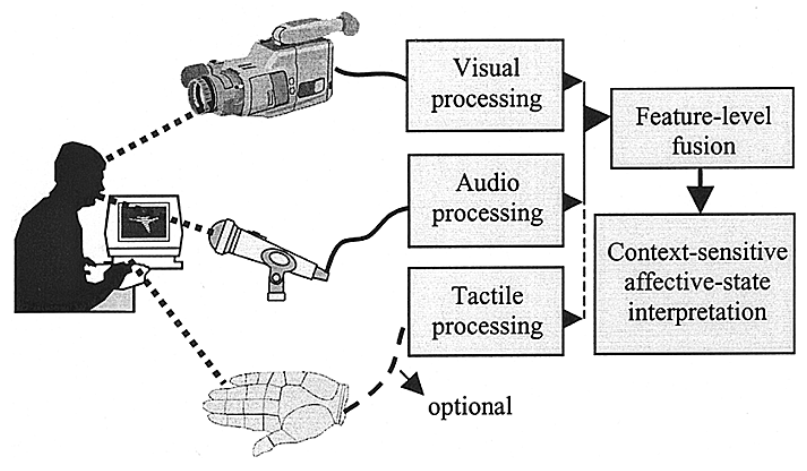
\includegraphics[width=0.9\columnwidth]{figures/Architecture}
  \caption{Architecture of automatic human affect analyser utilising fusion of approaches.}~\cite{pantic2003toward}~\label{fig:figure3}
\end{figure}

\subsection{Research into the role of light on mood and emotion}

A number of commercially available devices and academic studies have utilised the mediums of light and colour to enhance users sensory experience, room ambience and subsequently the mood of users~\cite{flores2017effect, kuijsters2011improving, kuijsters2015lighting}. Dutch researchers, Kuijsters, Reidi et al. were able to affectively intensify daily experiences for elderly and vulnerable care home occupants using colour-enhanced lighting. Indeed, they manually provided cosy ambiences to reduce elderly participants anxiety and an activating ambience to stimulate arousal~\cite{kuijsters2015lighting}. This study proves that a multimodal RGB LED lamp could serve its purpose by both enhancing users affective experience and improve on Kuijster et al.’s findings as the device will function both automatically and autonomously. Further underlining this, Kujisters et al. conclude, “we envision an adaptive ambience creation platform that can automatically adapt” – the proposed RGB LED lamp and multimodal affect-sensitive computer software will help directly fill this void~\cite{kuijsters2015lighting}.

An oft-cited study by Valdez et al. found that colours had definitive effect on the emotion of participants~\cite{valdez1994effects}. Using the PAD model blue, blue-green, green, red-purple, purple and purple-blue were the most pleasant hues~\cite{valdez1994effects} (see figure 2). With green-yellow, blue-green and green the most arousing whereas purple-blue and yellow-red amongst the least arousing~\cite{valdez1994effects}. Although further positive evidence for the potential effectiveness of the RGB LED lamp – Valdez et al.’s study is limited by the PAD model, which perhaps underplays the significance of their findings. Nontheless within experimental psychology, Valdez et al.'s research was entirely original at the time -  containing a sizable, coherent and specific dataset on influencing postive emotions within users utilising colour (figure 2). Significantly, this research has spawned a number of other critical studies into the affective influence of colour and coloured lighting on users~\cite{han2017effects, jo2014smart, kim2014study, lee2019effects, wardono2012effects, yang2015lighting} - consequently it is highly suitable research for helping develop the Turrellian RGB LED.

For instance, a larger and more diverse study by Kuller et al. utilised Valdez’s research and successfully adapted work environments lighting colour and conditions over a year within four different countries~\cite{kuller2006impact, kuller2009color}. They found that workers were most productive and positive and when lighting was not too bright (under 2000 lux) and too dark (above 500 lux)~\cite{kuller2006impact, kuller2009color}. In addition, mood was most positive amongst workers in colourful environments~\cite{kuller1986physiological}.

\subsection{Similar IoT light devices to the Turrellian RGB lamp}

Three commercial devices similar to the Turrellian RGB LED lamp include the Dyson Lightcycle~\cite{Dyson01}, Phillips Hue~\cite{Phillips01} and Nanoleaf light panels~\cite{Nanoleaf01}. Dyson’s LED Lightcycle auto-adjusts depending on age of user, tasks, senses motion and uses a 32-bit microprocessor to continually interpret daylight data to render the LED close to daylight colours~\cite{Dyson01}. Contrastingly, the most popular competitor device, the Phillips Hue is a line of colour changing 800 lumen LED lamps, strips and bulbs controlled wirelessly from Apps, vocally with Alexa or Google Assistant and configurable with iOS HomeKit~\cite{Phillips01}. Lastly, Nanoleaf Inc. are a diverse range of multicoloured LED light panels – integrable with assistant software and touch sensitive~\cite{Nanoleaf01}. 

These IoT devices differ enormously in terms of specifications, pricing, and market share. At the time of writing, the Phillips Hue is by far the most popular and successful smart IoT LED light device with the range reporting yearly revenues of almost €600 million~\cite{Phillips02}. The success of the Phillips Hue is potentially as a consequence of the breadth of its range and array of price points thus catering to a wide spectrum of potential customers in contrast to competitors~\cite{Phillips01}. Similarly, much like its competitors the Hue adjusts brightness based on time of day, can provide visual notification for users incoming Uber rides and can turn lights on with motion detection at predefined times – helping abate home burglaries~\cite{Phillips01}. 

Although not part of a broader range of lighting products and a newcomer within lighting markets, the Dyson Lightcycle offers eponymous elegant and aesthetic design. Intriguingly unlike competitors, the Lightcycle fails to offer a wide spectrum of colours and instead sticks to white hues. Furthermore, the price point of the Lightcycle is quite high at RRP over £500~\cite{Dyson01}. Former Kickstarter start-up Nanoleaf offers an intriguing coloured range of LED light panels. Unlike the other devices, Nanoleaf light tiles can be built up into large displays offering the canvassing potential and portability for large commercial installations. Additionally, Nanoleaf differs from its commercial counterparts as an emerging start-up rather than large enterprise with a more niche subset of retail customers~\cite{Nanoleaf01}. In particular Nanoleaf is commonly used for backlighting purposes for game consoles or televisions~\cite{Nanoleaf01}.

All devices fundamentally differ from the Turrellian RGB LED lamp as none are tethered to users’ affective state or offer mood enhancement. Rather the devices offer a more functional purpose – providing ambient lighting on command. This design oversight is all the more surprising with the numerous research papers and art features exploring the role of light, colour, and affect-sensitive computing towards improving user’s mood~\cite{lee2019effects, wardono2012effects, yang2015lighting}. Perhaps the difficulty of affect-sensitive computing IoT devices deters designers from further exploring mood-enhanced LED light - particularly designing autonomous instead of on-command devices. Yet as noted in the ensuing sections, this proposal supports the position that utilising embodied and scaffolded perspectives of the mind should admonish some of these preconceived difficulties. 

\subsection{Journaling applications similar to the RGB lamp GUI}

Several mindful applications are similar to the Turrellian RGB LED lamp GUI and journaling parser. With respect to journaling, the application Reflectly utilises artificial intelligence to help users’ structure and reflect upon their daily thoughts and problems~\cite{Reflectly01}. Reflectly tracks users’ moods, content progress and offering personalised motivational content. Reflectly has an aesthetically desirable UI. Yet aside from collecting data Reflectly, unlike the proposed Turrellian RGB LED, does not collect any physiological data or positively orientate user’s hardware and environment~\cite{Reflectly01}.

\subsection{Towards a physiological, embodied and scaffolded approach to MHCI and affect-sensitive computing}

Despite the secondary role of physiological affect sensors as mentioned earlier in the taxonomy. In fact, automated physiological affect sensing is a strong and undervalued modality which should be used for future multimodal affect-sensing computer systems because of three clear reasons. Firstly, Pantic et al.’s criticism, which centred on the discomfort of wearable computer devices no longer holds~\cite{pantic2008human, pantic2003toward, 6634207}. Secondly, studies and research into physiological affect sensing holds the most feasibility aside from text-based sentiment analysis~\cite{goshvarpour2017fusion, goshvarpour2017indices, goshvarpour2017discrimination}. Thirdly, insights from scaffolded affective cognition hold exciting future potential for physiological or embodied approaches towards affect-sensitive multimodal computing~\cite{colombetti2015scaffoldings}. 

Potentially, Pantic et al. were unable to foresee the continued exponential growth of Moore’s Law~\cite{lundstrom2003moore} and advent of more non-intrusive, comfortable sensors and wearables for accurate physiological data~\cite{chen2012making, pantic2008human}. Indeed, the demand for smart, ergonomic and non-intrusive wearable body sensors has grown in prominence~\cite{chen2012making}. From mobile devices~\cite{rodgers2014recent}, watches~\cite{kim2015acceptance}, smart running trainers~\cite{hurford2009types}, to even jewellery~\cite{ju2015smart} – often-AI driven “smart” physiological sensors designed to collect data on sleep, heartrate, steps, respiration, bodily posture and plenty more. User requirements and competitive markets will help to ensure these devices get smarter, less obtrusive and collect better physiological data on their users, which can then subsequently be fed to affect-driven computer devices such as the proposed Turrellian RGB LED. 

Although this paper accepts that a broad fusion of approaches discussed in the taxonomy is ultimately most ideal (see figure 3), physiological data collection should become more central in future developments towards affect-sensitive multimodal computing. Physiological approaches avoid the potential difficulties of facial recognition and auditory approaches as they are easier to employ automatically and accurately. Research by Goshvarpour et al. using heart rate and respiratory volume demonstrated affective classification rates of up to 92 percent (sensitivity: 95 percent and specificity: 83.33 percent) utilising heart rate variability and pulse rate alone~\cite{goshvarpour2017fusion}. Also, high accuracy was observed in research by Piana et al. of 84.7 percent for recognition of boredom, pain and surprise emotions utilising physiological signals~\cite{piana2014real}. Even body posture and movement has also been recognised as an effective expressive modality for human emotion. Li et al. utilising Microsoft Kinect found that a walker’s gait was successful in determining participants emotional state~\cite{li2016emotion}. Accordingly, the proposed Turrellian RGB LED should perform well in affect-detection because it will combine many of the above physiological approaches. 

There is further reason to support physiological and embodied approaches to multimodal affect sensing for computing and smart IoT devices. Many prominent neurologists and enactivists have argued that emotion is embodied and induced by bodily events~\cite{colombetti2008feeling}. Emotion-theorists William James and Carl Lange argued that autonomic bodily changes precede our emotional experiences~\cite{james1994physical, lange1885om}. Indeed, James convincingly states that emotional experience abstracted from all physical bodily feelings is simply nothing but “feelingless cognition”~\cite{james1894discussion, james1922emotions}. In addition, Levenson, Ekman and Friesen found that for the six basic emotions each of these corresponds to a unique bodily pattern~\cite{levenson1990voluntary, prinz2004gut}. Therefore, physiological affect-sensing has been widely recognised even by researchers primarily utilising visual depictions of facial actions for studying emotion.

Other compelling support for physiological approaches becoming central to the design and implementation of affect-sensitive multimodal computer systems and IoT devices includes research into unconscious emotion~\cite{scarantino2010insights, winkielman2004unconscious}. Within Scarantino’s blindfright experiments he was able to activate subject’s neurophysiological fear system – inspiring consciously unfelt yet empirically measurable physiological, facial and bodily changes coherent with the emotion of fear~\cite{scarantino2010insights}. Indeed, in response to unseen stimuli and without conscious awareness subjects demonstrated: enhanced SCRs, potentiated startle reflex and differential amydala activation~\cite{scarantino2010insights, winkielman2004unconscious}. Enabling the development of computer systems which can automatically respond to emotion sourced from bodily change and even anticipate users emotional state from their unconscious bodily changes and emotions~\cite{scarantino2010insights, smith2016unconscious}. Hence, it will be exciting to determine if the RGB LED offers anticipatory performance.

Lastly, research from emotion theorists Colombetti and Krueger into scaffolded emotion theory has demonstrated exciting potential for the RGB LED and other affect-sensitive computer devices~\cite{colombetti2015scaffoldings}. Extending Sterelny’s scaffolded framework for the mind they have found strong empirical and phenomenological evidence that affective states are environmentally supported~\cite{sterelny2010minds, sterelny2004externalism}. With this consideration, the proposed Turrellian RGB LED should certainly help improve user’s mood by providing a comforting environment conducive to users present mental state. Indeed, MHCI researchers have been keen to emphasise the importance of affect-sensitive computer devices to help improve users experience, mood and mental health~\cite{de2013predicting, fitriani2007multimodal, 5771346}. Particularly with modern lifestyles centred on high computer screen time and usage~\cite{MedicalNews03, MedicalNews01, MedicalNews02}. 

\section{Research hypotheses}

The ability to succinctly recognise the affective states of an individual we are communicating with is a key facet of human emotional intelligence. Consequently, MHCI designs must simulate this feature of human to human social communication to eventually ensure more human-like, effective, and efficient computer interfaces and devices~\cite{fitriani2007multimodal}. Indeed, research from Rothkrantz et al. finds that people consider computers as social agents with whom “face-to-(inter)face” interaction may be most amenable~\cite{pantic2003toward}. Thus, MHCI systems capable of responding appropriately to users’ affective feedback are likely to be perceived as more natural, efficacious, persuasive, and trustworthy~\cite{pantic2003toward}.

The following section will discuss this proposals research hypotheses. The hypotheses envision that affective ambiences created by the RGB LED will alter and improve user’s mood. Furthermore, the devices’ awareness of users’ affective state will demonstrate progress in the development of more socially amenable and better computer systems. 

\subsection{Hypotheses evaluation}

This paper offers insights from building an affect-enhanced RGB LED lamp utilising tightly synchronised body sensors and a self-journaling application to gauge users’ affective signals. Lastly for evaluation purposes, a control lamp will be used to contrast with my device – a lamp which changes colour every five minutes without user feedback to determine that my RGB LED device has worked effectively and that the affect driven colour changes are having the desired impact on their users.

Specifically, I have formulated two hypotheses. The first hypothesis centres on quantitative data collection – precisely collecting data on users physiological and thus emotions rendered in the presence of the LED lamp. Contrastingly, my second hypothesis focuses on qualitative evaluation and user feedback including whether users are supportive of the device and would consider purchasing one:

(1) The affective or physiological state of a person will be significantly altered by the Turrellian lamp’s light changes.

(2) Users will be able to consciously recognise the effect that the lighting manipulation is having on their affective state. Furthermore, the Turrellian lamp will be better received than the control lamp by its cohort of users.

Data collected in respect to my first hypothesis will demonstrate the physiological changes of users rendered in the presence of the LED lamp. For instance, measurable changes in heart rate, skin conductivity and palpitation. As previously noted, coloured light changes to render positive emotion for users will be determined by the colour palette’s documented by psychologists Valdez and Biggam et al.~\cite{biggam2006progress, valdez1994effects}. 

With regards to the second hypothesis, Sterelny’s scaffolded or extended-mind theory teaches that our affective states are environmentally supported~\cite{sterelny2010minds, sterelny2004externalism} consequently it is fully expected that the Turrellian LED will promote a positive user-experience. Encouraging self-noticeable positive mental well-being and a desirable environment or setting. In contrast, the control lamp will not display the same levels of effectiveness within its cohort of users because its changes will be automatic instead of being guided by users physiological state. Presently an independent nursery franchise in London has agreed to testing my device to help develop a better learning environment for their pupils and staff.

\subsection{Research objectives}

This research is focused on delivering computer hardware and software affectively sensitized to its user utilising insights from the latest MHCI research, neuroscience, psychology and ambience research into lighting and colour. Indeed, disparate fields of study can increase our understanding of human communication modalities thereby promoting a paradigm shift from PC applications to services and devices delivered in a more human-centred, affectively sensitive, and multimodal manner. 

\subsection{Summary of core objectives}

This paper has three core objectives. Firstly, to build the RGB LED device. Secondly, to collect physiological data from users to provide data towards evaluating the first hypothesis. Thirdly, to document and evaluate user’s response to the device, determine if it is well-received and holds potential to improve user’s quality of life.

\subsection{Broader objectives}

Broader objectives of this research include facilitating the development of more and better multimodal affect-sensitive computer systems. Commercially, we have seen increasing demand for smart lighting systems most notably, the Philips Hue~\cite{Phillips01} and mental health or mindful applications for instance, Reflectly~\cite{Reflectly01}, Calm~\cite{Calm01} or Headspace~\cite{Headspace01}. Just like these applications, this research paper seeks to promote the development of computer devices which improve user’s quality of life, mood and machine interaction as well as enhance future software and hardware research within affect-sensitive computing. Crucially this papers research will be fully accessible utilising opensource libraries and hardware. 

Inspired by the phenomenological work of artist and architect Turrell another broader objective of the RGB LED lamp is that it is designed to bridge the gap between mindfulness applications and smart lighting systems – improving users’ day-to-day quality of life. Features of the lamp GUI will include providing light recipes for users’ daily routines, or tasks and providing personalised lighting dependent on specific age and situational needs. In addition, the lamp will render coloured and lumen of lighting conducive to the users’ mood based upon physical emotive feedback and reflective journaling. Establishing ambience to help both day-to-day or with more specific mindful tasks such as guided meditations in order to help abate users daily stress and anxiety.

\section{Proposed Approach}

This section will sequentially discuss and evaluate this papers’ proposed approach to achieve the core objectives outlined earlier and milestones timelined in the 6-month gantt chart outlined on  landscape below as figure 4. Before presenting a full risk table for the project - see table 1 (below figure 4). 

\section{Discussion of gantt chart}
\subsection{RGB LED hardware development}

For this paper there are four clear steps in the hardware development cycle (see figure 4) before the milestone of prototype built is achieved. Step one will involve wiring and soldering RGB LEDs to a single-board microcontroller. Single-board microcontrollers such as the Raspberry Pi have been chosen to enable the device to be opensource and accessible for other MHCI researchers. RGB LEDs will be used to make the device produce the colour ranges formulated by psychologists Valdez and Biggam et al. – permitting research towards my first hypothesis on the role of light and mood~\cite{biggam2006progress, valdez1994effects}.

Step two will concentrate on making the RGB LED device communicative. This will be achievable by adding relevant Wi-Fi and Bluetooth modules to the single-board microcontroller. Step three of the hardware development cycle will focus on having the device receive data from physiological monitors from wearable processors. Physiological sensors will tether the device to users’ affective signals – providing research and data for my first hypothesis and for affect-enhanced computing research. Lastly, step four centres on building an encasing for the IoT device. Generating a professional encasing utilising a 3D printer would be an aesthetic and desirable feature, although may be challenging during the present international crisis.

\subsection{Integration of software and GUI application}

After hardware development, agile and intently user-focused software development will compromise the dominant approach for developing RGB LED software~\cite{abrahamsson2017agile, cockburn2006agile}. Presently, agile software development is considered the optimum approach to enable fast development and client satisfaction however this development process will ultimately be evaluated~\cite{abrahamsson2017agile}. Three key procedures must be mitigated within the RGB LED software development cycle before the software-harware integration milestone is achieved. Firstly, effective programming of the microcontroller to produce lighting and process physiological data input – enabling constant calibration and coherent lighting for the user as well as providing data for my first hypothesis. Secondly, integration of an emoji-based parser and emoji or journal application to determine the written affective signals of the user for the RGB LED utilising APIs such as Microsoft Azure. Thirdly and finally tying the three procedures together with the development of a GUI application to enable ease of use. 

\subsection{User experience testing of the RGB LED}

Once the Turrellian RGB LED has been fully developed as outlined in the seven key steps noted in figure 4 – testing of the effectiveness of the device can commence. Resolution and data collected for my two hypotheses will be evaluated and determined. A user-centric approach will be adopted in the testing of the device. Users will be aided through wiring physiological sensors and provided with ample time to self-journal their present affective state through the RGB LED GUI journal. Users will be given substantial exposure to the RGB LED for at least twenty minutes.

After the timed session, all physiological data will be saved – users will be notified of any significant physiological changes and provided with a feedback form and five-minute interview time for additional comments and thoughts. Maximum participant time will be thirty minutes. Participants will be provided with my personal contact details if they form any thoughts later upon further reflection.

\subsection{Ethical considerations}

A full ethics application will be submitted to Faculty of Engineering Research Ethics Committee for approval. Participants will be provided with a full information sheet in advance of the experiment. This document will ask for approval to record participants experience utilising the lamp, preceding comments and feedback on the device. 

Consent will be taken in the form of a signature and also video recording. Participants can drop out of the experiment at any time. All data gathered from experimentation will be securely retained on an encrypted external drive which only the student and supervisor has access. Personal identifying information will not be collected instead arbitrary participant numbers will be stored for identification. 

Formal experimentation (ie. wiring of physiological sensors) will strictly involve adults over the age of eighteen and United Kingdom residents. All information recorded will be confidential, with anonymous interview data encrypted (per University of Bristol Policy) and stored by the student on a password-protected computer system only accessible by the student. Importantly, the nursery chain has provided consent for coloured lighting rendered by the device to be exposed to its pupils with only adult staff having physiological data tracked. 

\subsection{Data analysis of findings}

There is a widespread and useful variety of open source libraries and applications to perform analysis of physiological data collected. Open source API’s for IOTs and small-scale projects such as Thingspeak which utilises MATLAB and Simulink will prove invaluable for collecting and visualising data from the Turrellian RGB LED UX testing~\cite{Thingspeak01}. To summarise and conclude, physiological data and textual input will be dually analysed for affective sentiment, which in turn will determine the colour rendered of the LED RGB light.


\subsection{Limitations and responses}

There are three limitations of this proposed research. Firstly, the reliance on UX testing to evaluate the effectiveness of the device and hypotheses proposed. Indeed, in the present global circumstances with the Coronavirus pandemic it is unlikely enough user testing will be conducted to conclusively determine if the device is successful as an affect analyser or at improving users mood. Nonetheless, this research expects to gain enough data to reach initial conclusions, which can be evaluated and supported by future research within multimodal affect-senstive computing. 

Secondly, another limitation is that the device could be better designed with more affect-sensors (see figure 3) - perhaps even a camera to perform facial analysis of users as well. In response to this, although more sensors may be desirable, it would be a highly complex a task given the timescale of the project. Therefore the lamp will be configured to use physiological (tactile) sensors and a journalling application, which are most significant for affect detection as outlined in the literature review. Thirdly, potentially a lamp is perceived to be a "weak" IoT device for improving users mood. With regards to this, scepticisms should be mitigated by numerous studies from psychologists or ambience researchers and the incredibly immersive lightscapes of Turrell - yet the effectiveness of the device will be evaluated.   

\subsection{Concluding remarks and significance}

The research proposed expects to acheive two objectives. Initially, to design and evaluate a Turrellian RGB LED lamp through UX testing and secondly to utilise the device to provide further research into developing successful multi-modal affect-senstive computer systems. Furthermore, this research holds significance within two crurcial contexts. Firstly, if deemed effective by thorough UX testing, the Turrellian lamp could help pave the way for better designed and more human-centred computer technolgies and IoT devices, which enrich users mental health and improve man-machine interaction. Secondly, for academia the Turrellian RGB LED lamp will contribute towards the academic research outlined in the literature review, particularly MHCI and ambience research. Undeniably, the lamp will challenge many approaches from other MHCI researchers by utilising a strongly embodied, physiological and tactile modus for affect-detection. 



\pagestyle{empty}
\begin{landscape}
    \begin{figure}
    \centering
\vspace*{-1cm}
\hspace*{-3cm}
        \begin{ganttchart}[%Specs
            y unit title=0.4cm,
            y unit chart=0.5cm,
            canvas/.style={fill=none, draw=black, line width=.75pt},
            vgrid,
            title label anchor/.style={below=-1.6ex},
            title left shift=.05,
            title right shift=-.05,
            title height=1,
            title/.style={fill=none},
            title label font=\bfseries,
            bar/.style={fill=barblue},
            incomplete/.style={fill=white},
            progress label text={},
            bar height=0.7,
            group right shift=0,
            group top shift=.6,
            group height=.3,
            group peaks height=.2]{1}{36}

            %labels
            \gantttitle{Six-month timeline and project milestones}{36}\\
            \gantttitle{April}{6}
            \gantttitle{May}{6}
            \gantttitle{June}{6}
            \gantttitle{July}{6}
            \gantttitle{August}{6}
            \gantttitle{September}{6}\\

            % Parameter Selection
            \ganttgroup{Research Proposal}{2}{9}\\ %elem0
       	 \ganttmilestone{Business franchise for UX testing found}{3}\\
            \ganttbar[progress=100]{Development}{2}{9}\\
            \ganttbar[progress=90]{Hardware sourcing}{2}{9}\\
            \ganttmilestone{Proposal submission}{9}\\\\

            % Testing equipment
            \ganttgroup{Hardware Development}{10}{18}\\ %elem0
	 \ganttbar[progress=0]{Wiring / soldering}{10}{14}\\
            \ganttbar[progress=0]{Communicative features}{10}{11}\\
	 \ganttbar[progress=0]{Physiological sensors}{14}{16}\\
	 \ganttbar[progress=10]{Encasing construction}{16}{18}\\
            \ganttmilestone{Prototype built}{18}\\\\

            % Testing equipment
            \ganttgroup{Software Integration}{17}{23}\\ %elem0
            \ganttbar[progress=0]{Microcontroller programming}{17}{19}\\
            \ganttbar[progress=0]{Parser development}{18}{20}\\
            \ganttbar[progress=0]{GUI application}{20}{23}\\
            \ganttmilestone{Software-hardware integrated}{23}\\\\

           % Testing equipment
            \ganttgroup{Prototype Testing}{22}{25}\\ %elem0
            \ganttbar[progress=0]{Supervisor Feedback}{24}{25}\\
            \ganttmilestone{Completed Turrellian RGB LED}{25}\\\\

           % Testing equipment
            \ganttgroup{Scheduled UI and UX testing}{26}{27}\\ %elem0
            \ganttbar[progress=0]{Data collection}{26}{27}\\
            \ganttmilestone{Testing completed}{27}\\\\
	
	 % Testing equipment
            \ganttgroup{Dissertation writing}{12}{33}\\ %elem0
            \ganttmilestone{Ethics application}{10}\\
            \ganttmilestone{Literature review completed}{20}\\
            \ganttbar[progress=0]{Data analysis}{27}{28}\\
            \ganttmilestone{Integration and evaluation of findings}{29}\\
            \ganttbar[progress=0]{Supervisor redrafting}{30}{31}\\\\
            \ganttmilestone{Dissertation submission}{32}\\

            %relations 
            \ganttlink{elem1}{elem4}
            \ganttlink{elem4}{elem10}
            \ganttlink{elem7}{elem8}
            \ganttlink{elem13}{elem14}
            \ganttlink{elem10}{elem15}
            \ganttlink{elem15}{elem18}
            \ganttlink{elem18}{elem21}
            \ganttlink{elem18}{elem21}
            \ganttlink{elem23}{elem24}
            \ganttlink{elem24}{elem25}
            \ganttlink{elem25}{elem26}
            \ganttlink{elem26}{elem27}
            \ganttlink{elem27}{elem28}


        \end{ganttchart}
    \caption{Gantt chart of Turellian RGB LED proposed approach 2020. (Please note: blue bars denote progress made and diamonds milestones)}
    \label{fig:Gantt2014}
    \end{figure}
\end{landscape}


\newpage{%
    \clearpage% Flush earlier floats (otherwise order might not be correct)
    \pagestyle{empty}
    \begin{landscape}% Landscape page
  \begin{tabular}{c c c c c c}
    {\textit{Risk}}
& {\textit{Probability}}
& {\textit{Severity}}
& {\textit{Reason}} 
& {\textit{Consequence}} 
& {\textit{Mitigation}} \\
    \midrule
Sourcing Hardware & Low & High & 
$\begin{matrix} \text{Supply chain disruption due to the} \\ \text{Coronavirus crisis may cause} \\ \text{disruption – preventing access} \\ \text{to necessary electronic parts.} \end{matrix}$ & $\begin{matrix} \text{Hardware stymied} \\ \text{and lacking full} \\ \text{development.} \end{matrix}$ &
$\begin{matrix} \text{Supply chain disruption due to the} \\ \text{Coronavirus crisis may cause} \\ \text{disruption – preventing access} \\ \text{to necessary electronic parts.} \end{matrix}$\\
    \midrule
Hardware Issues& Medium & Medium &
$\begin{matrix} \text{I am a novice at } \\ \text{soldering thus potentially} \\ \text{could develop hardware} \\ \text{issues with soldering the} \\ \text{LEDs for prototyping of the} \\ \text{M5 stack.} \end{matrix}$ & 
$\begin{matrix} \text{Hardware breaks preventing} \\ \text{prototype objectives} \\ \text{from being accomplished.} \end{matrix}$ &
$\begin{matrix} \text{Support will be accessed from} \\ \text{experienced solder and} \\ \text{electronics repairman happy to} \\ \text{support during the} \\ \text{Coronavirus crisis.}\end{matrix}$\\
    \midrule
3D printed prototype & High & Medium & 
$\begin{matrix} \text{Due to the global Coronavirus} \\ \text{crisis it may be potentially} \\ \text{exceedingly difficult to find} \\ \text{and use a 3D printer for} \\ \text{prototyping designs} \end{matrix}$ & 
$\begin{matrix} \text{The end product is not} \\ \text{completely designed from} \\ \text{initial drawn prototypes.} \end{matrix}$ &
$\begin{matrix} \text{Will reconfigure designs} \\ \text{and purchase a pre-existing} \\ \text{marketplace light fitting} \\ \text{to create a functional display.} \end{matrix}$\\
    \midrule
Software Issues & Low & Medium &
$\begin{matrix} \text{Software may develop} \\ \text{compatibility issues or} \\ \text{even corrruption.} \end{matrix}$ & 
$\begin{matrix} \text{Reduction in work} \\ \text{efficiency and goal} \\ \text{acheivement.} \end{matrix}$ &
$\begin{matrix} \text{Ensure cloud backup of} \\ \text{all data and thorough use} \\ \text{of Git (agile development)} \\ \text{thus can effectively.} \\ \text{version control.} \end{matrix}$\\ 
    \midrule
Arranged User Testing Cancelled & Medium & High &
$\begin{matrix} \text{Firm which has agreed to} \\ \text{user test the device pulls} \\ \text{out due to Coronavirus} \\ \text{concerns and social} \\ \text{distancing rules.} \end{matrix}$ & 
$\begin{matrix} \text{Unable to provide} \\ \text{effective user evaluation} \\ \text{of the Turrellian} \\ \text{RGB LED.} \end{matrix}$ &
$\begin{matrix} \text{Will discuss and coordinate} \\ \text{a response with my} \\ \text{supervisor quickly and} \\ \text{efficiently.} \end{matrix}$\\
    \midrule
Personal Illness & Medium & High &
$\begin{matrix} \text{Both parents are key} \\ \text{workers. In particular,} \\ \text{my mother works closely} \\ \text{with NHS staff everyday.} \end{matrix}$ & 
$\begin{matrix} \text{Unable to work} \\ \text{due to ailment} \\ \text{or sickness.} \end{matrix}$ &
$\begin{matrix} \text{Have potential to be} \\ \text{tested and can mitigate} \\ \text{issues via support and} \\ \text{communication with the.} \\ \text{University of Bristol} \\ \text{and my supervisor.} \end{matrix}$\\
    \midrule
        \end{tabular}
        \captionof{table}{Full Risk Analysis table}% Add 'table' caption

\section{Risk analysis table overview}

In these difficult circumstances – evaluation of risk is an even more crucial process. Due to the present global conditions with the Coronavirus pandemic there are numerous risks overlooked by the following Risk Analysis table with low to medium probability and low to medium severity for my respective project. However, with the close support of my supervisor and the University of Bristol – these unforeseen uncertainties should be mitigated.

    \end{landscape}
    \clearpage% Flush page
}

\newpage

%%%%%%%%%%%%%%%%%%%%%%%%%%%%%%%%%%%%%%%%%%%%%%%%%%%%%%%%%%%%%%%%%%%%%%%%%%%%%%%

\section{Acknowledgments}

I would like to first and foremost thank the incredible help of my supervisor Dr Paul O'Dowd throughout these tough circumstances. His advice, thoughts and tireless work helped immensely in drafting this proposal. Additionally, I would also like to thank the support of fellow MSc student Nathan Cubbitt for lending LEDs and offering plenty of experienced microcontroller advice for this proposal. Lastly, my parents for there huge support - especially with providing financial support for the project so far. 

% BALANCE COLUMNS
\balance{}

% REFERENCES FORMAT
% References must be the same font size as other body text.
\bibliographystyle{SIGCHI-Reference-Format}
\bibliography{sample}

\end{document}

%%% Local Variables:
%%% mode: latex
%%% TeX-master: t
%%% End:
